\section{Results}


We present here the results of the example analysis. Figure \ref{fig:exploratory_analysis} shows the exploratory analysis where the simulated data are represented on the right and the distribution of the response variable is shown on the left.

\begin{figure}
\centering
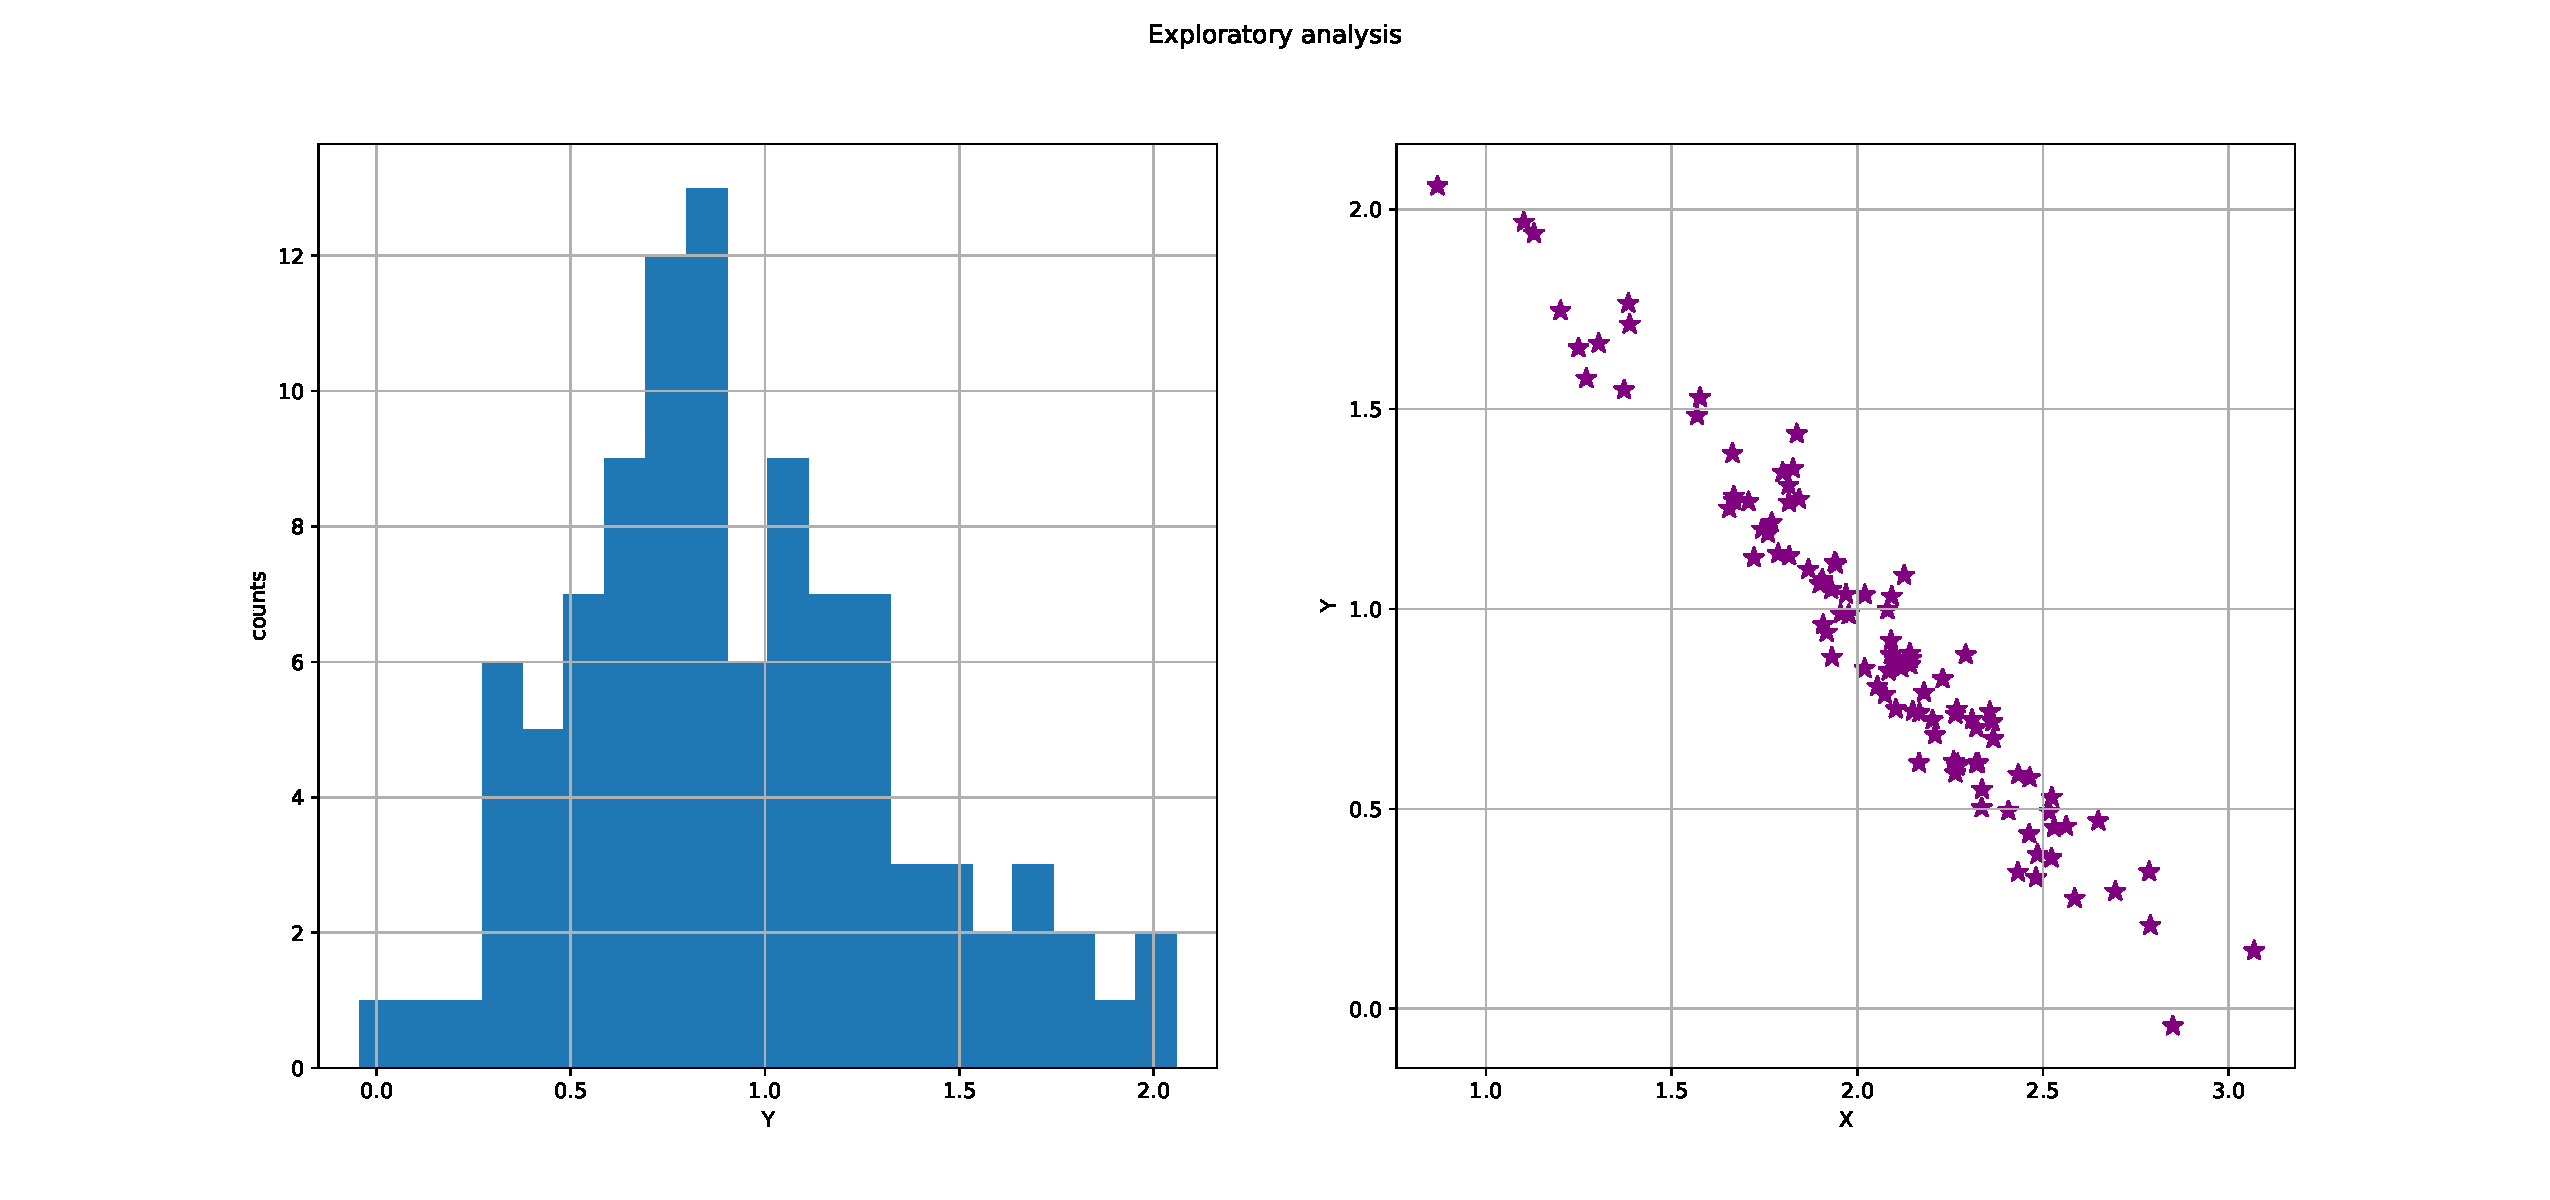
\includegraphics[width=\textwidth]{figures/fig_exploratory_analysis.pdf}
\caption{Exploratory analysis in python}
\label{fig:exploratory_analysis}
\end{figure}

Figure \ref{fig:linear_regression} shows the resulting simple linear regression. The figure on the left shows the fitted regression line where the estimated coeffcients fit very well the simulated coefficients on the python codes. The model presents a good fit as shown on the right figure. 

\begin{figure}
\centering
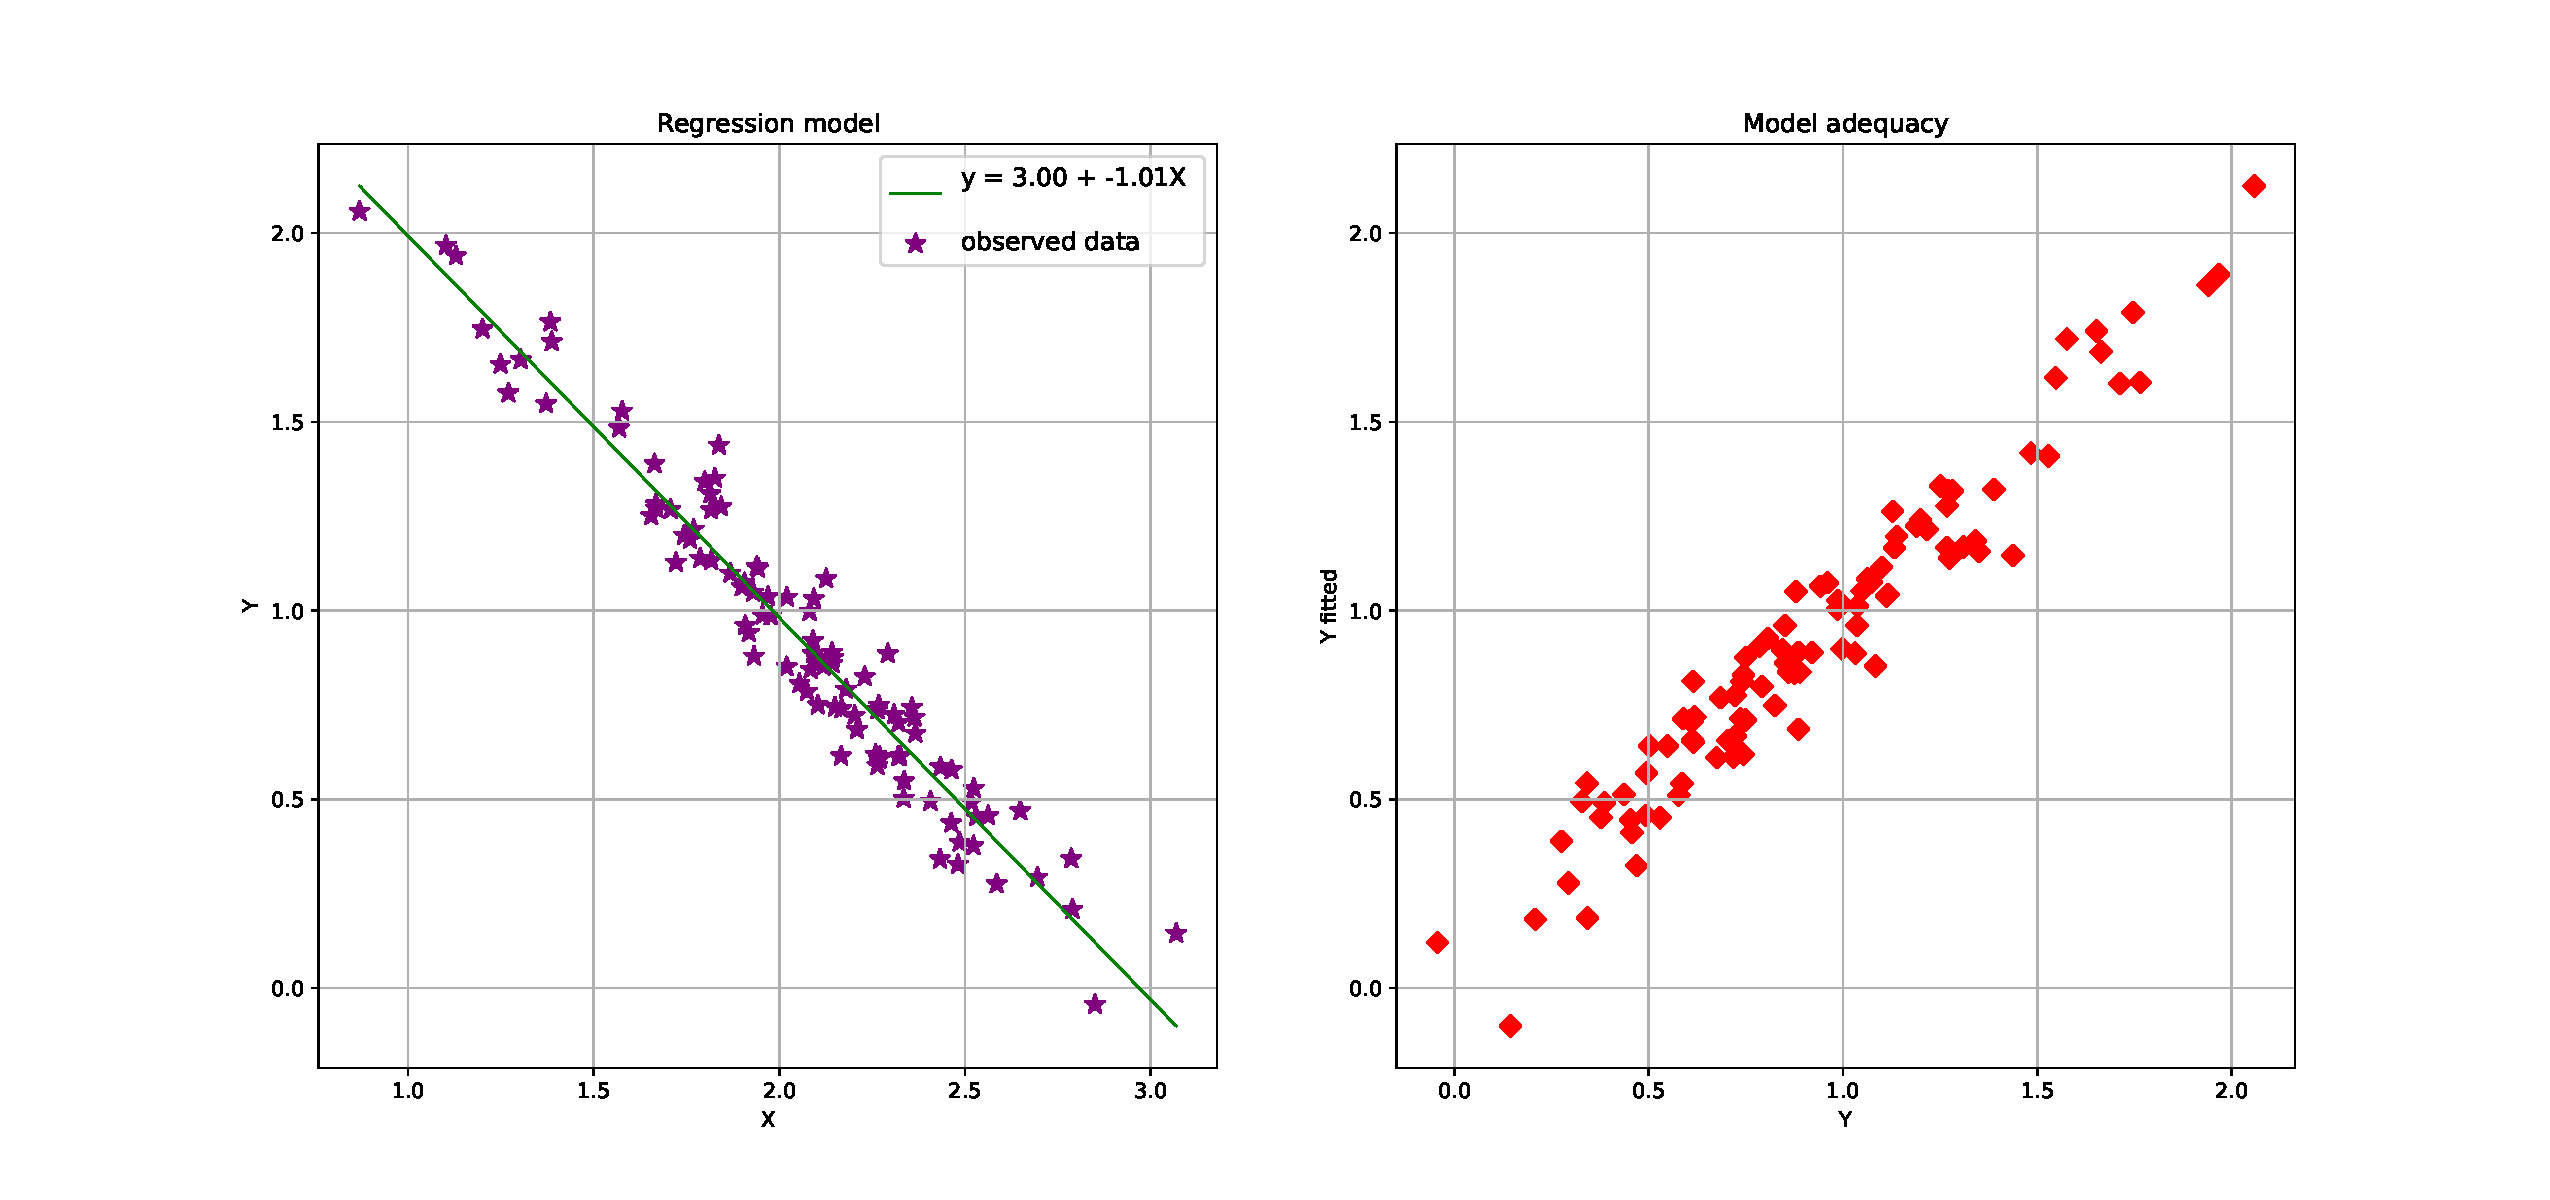
\includegraphics[width=\textwidth]{figures/fig_linear_regression.pdf}
\caption{Linear regression using scikit-learn}
\label{fig:linear_regression}
\end{figure}